% Automaton corresponding to the formula phi = exists P. (Sing(P) and not P
% \subseteq X)

\documentclass{standalone}

\usepackage{pgf}
\usepackage{tikz}
\usepackage{amssymb}
\usetikzlibrary{arrows,automata}
\usepackage[latin1]{inputenc}
\begin{document}
%\begin{figure}
% \begin{center}
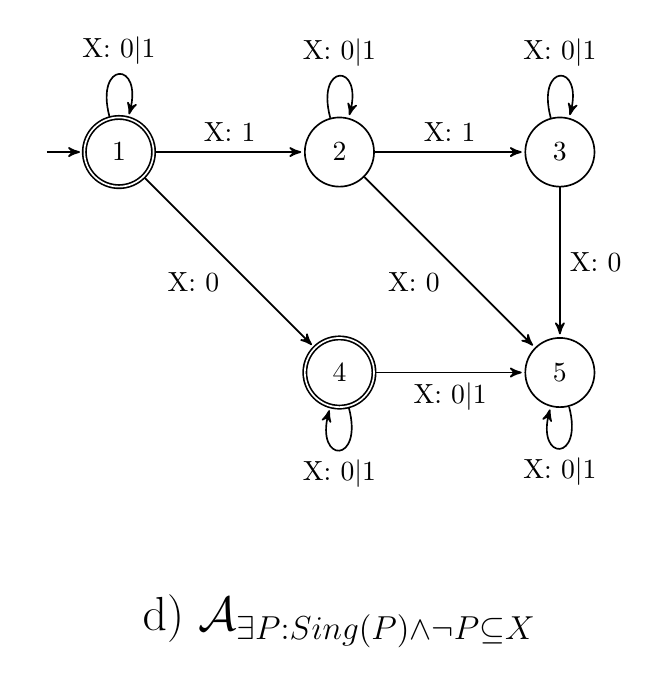
\begin{tikzpicture}[->,>=stealth',shorten >=1pt,auto,node distance=2.8cm,
                    semithick,initial text={}]
  \tikzstyle{every state}=[fill=none,draw=black,text=black]

  \node[initial,state,accepting] (A)                    {$1$};
  \node[state]         (B) [right of=A]       {$2$};
  \node[state]         (C) [right of=B]       {$3$};
  \node[state,accepting]         (D) [below of=B]       {$4$};
  \node[state]         (E) [below of=C]       {$5$};

  \path (A) edge              node {X: 1}   (B)
            edge [loop above] node {X: 0\textbar 1} (A)
            edge [below left]             node {X: 0}   (D)
        (B) edge              node {X: 1}   (C)
            edge [loop above] node {X: 0\textbar 1} (B)
            edge [below left]            node {X: 0}   (E)
        (C) edge [loop above] node {X: 0\textbar 1} (C)
            edge              node {X: 0}   (E)
        (D) edge [below]             node {X: 0\textbar 1} (E)
            edge [loop below] node {X: 0\textbar 1} (D)
        (E) edge [loop below] node {X: 0\textbar 1} (E);
        
    \node [below=5.5cm, align=flush center,text width=6cm] at (B)
        {
            \LARGE d) $\mathcal{A}_{\exists P: Sing(P) \wedge \neg P \subseteq X}$
        };
\end{tikzpicture}
% \end{center}
% \caption{Automaton $\mathcal{A}_\phi$ corresponding to the formula $\phi =
% \exists P. (Sing(P) \wedge \neg P \subseteq X)$}
%\end{figure}
\end{document}